\interlude[2]{Redefining QKD Success}
\section{Redefining QKD Success}

\newcommand*{\threePillarsSlide}{
  \begin{frame}{Three Pillars of passive Security}
    \begin{columns}[c]
      \begin{column}{.4\linewidth}
        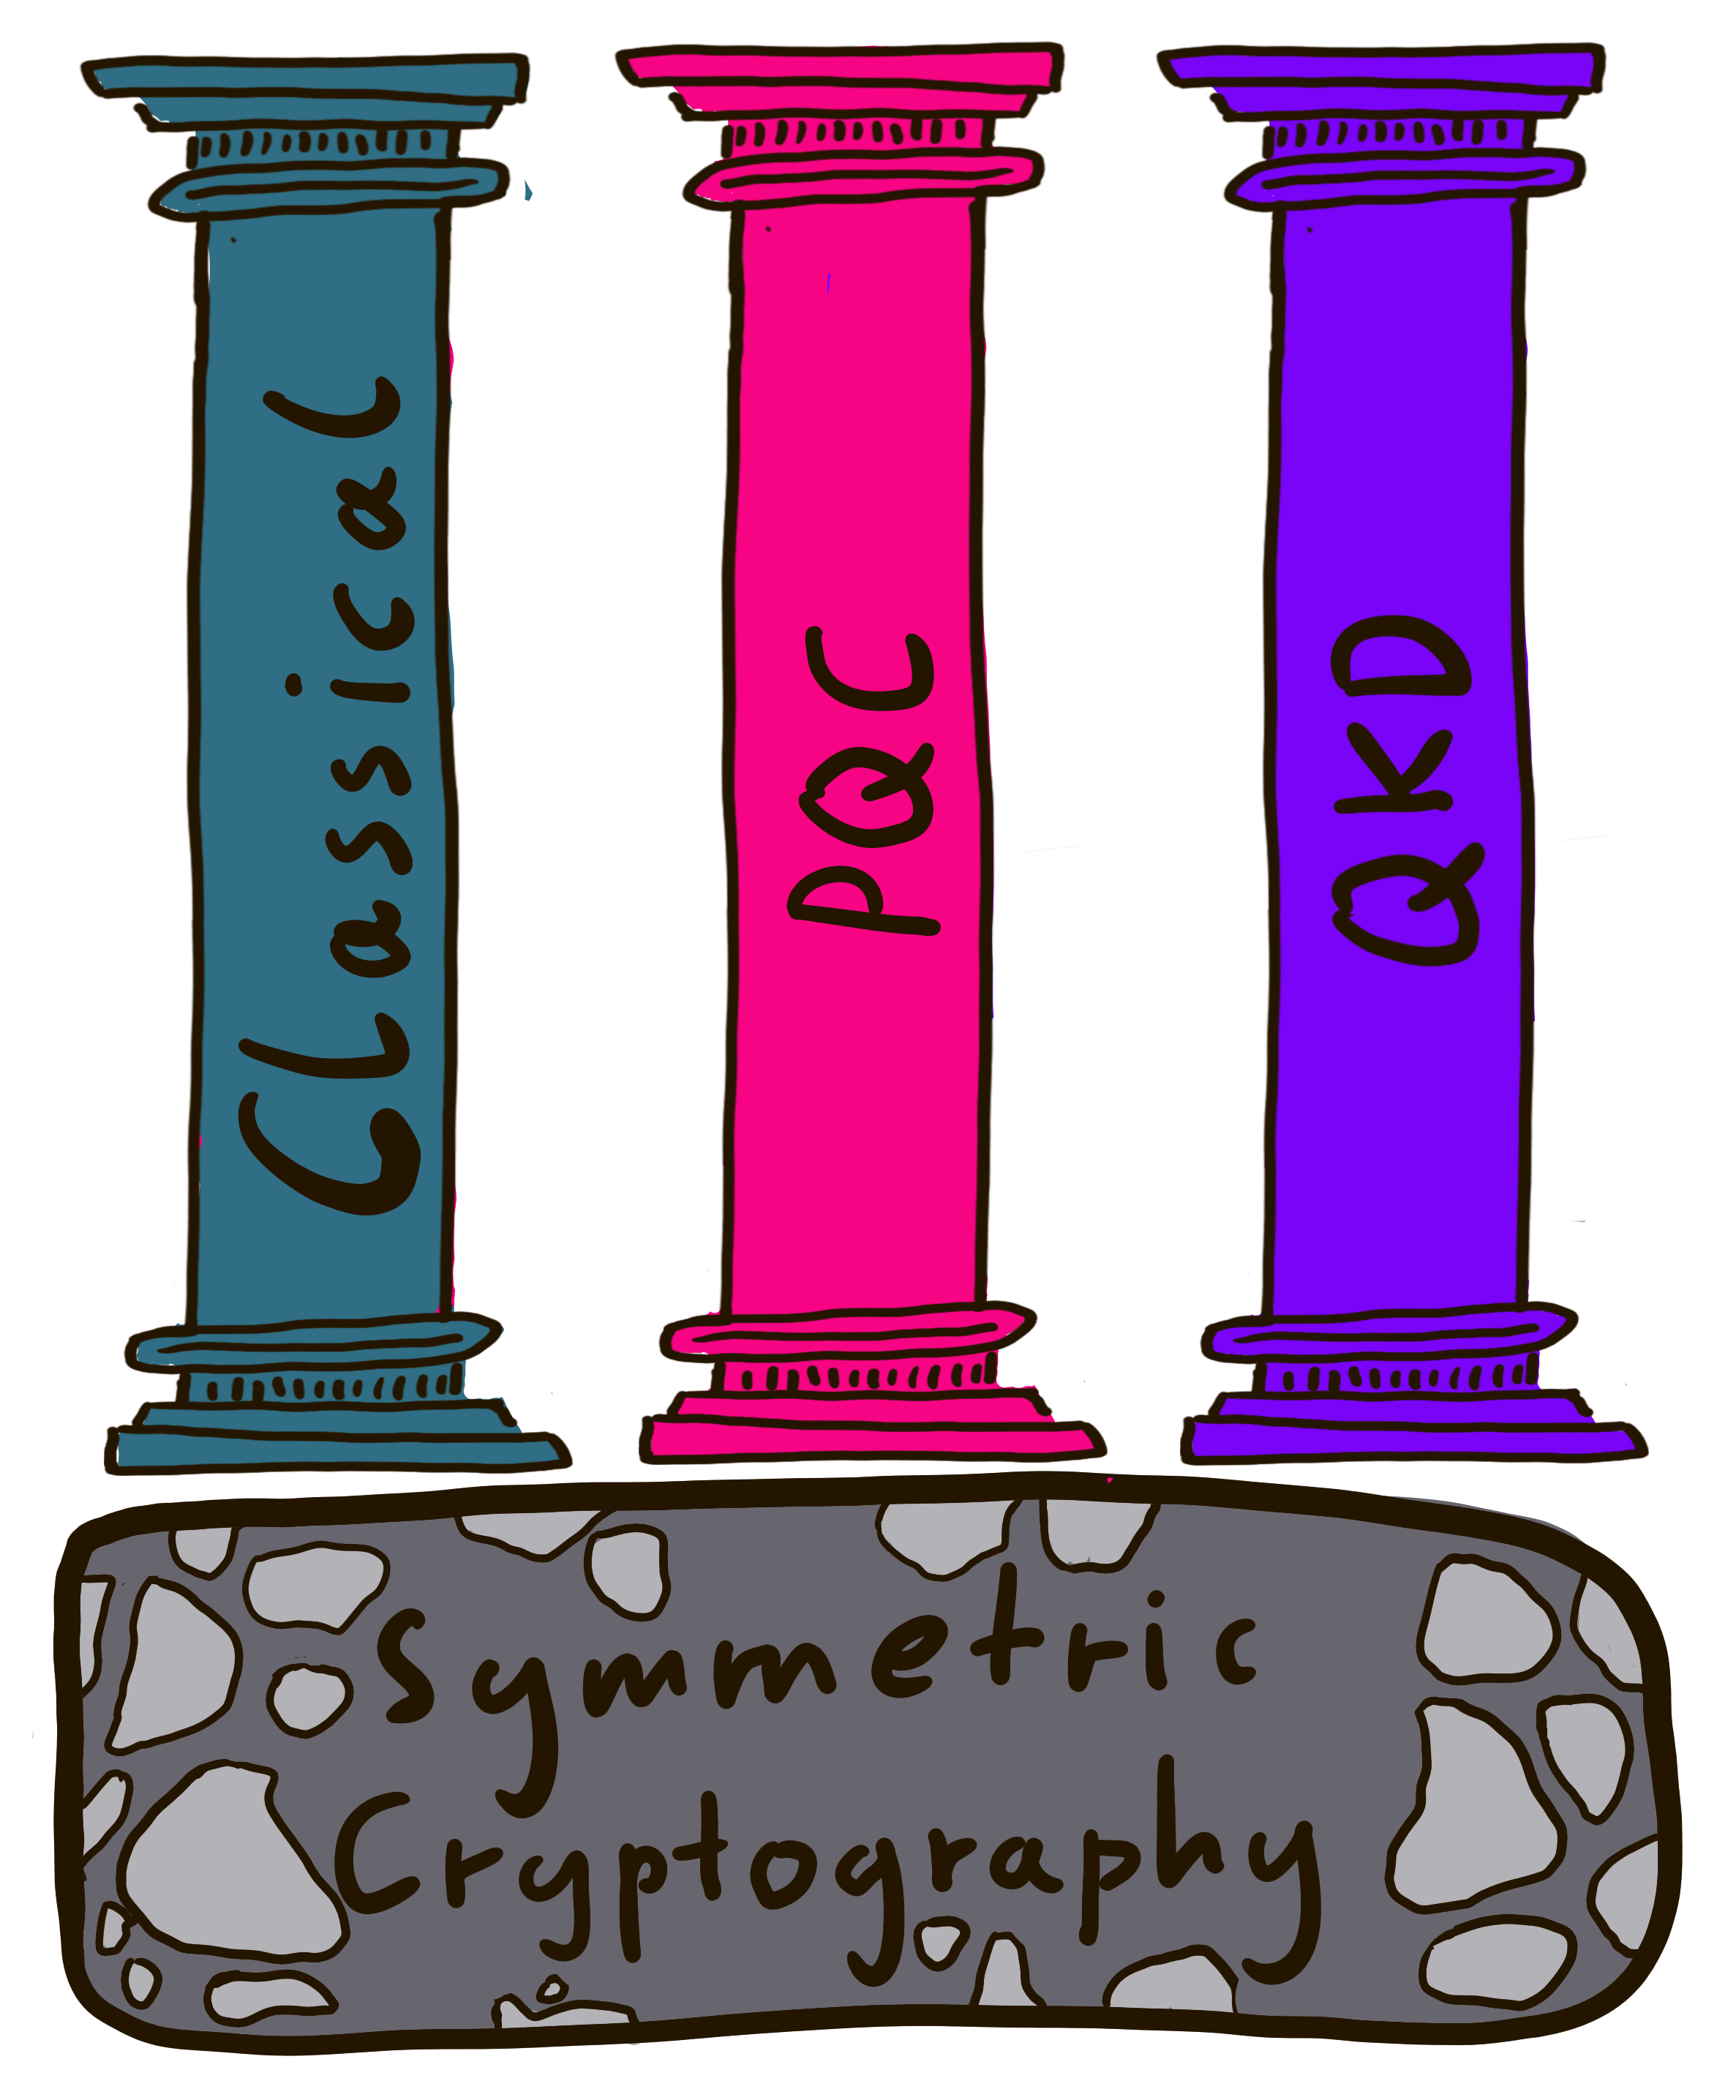
\includegraphics[height=\defaultframetextheight]{graphics/Three pillars of hybrid qkd.png}
      \end{column}

      \begin{column}{.5\linewidth}
        \stretchcolumn{
          \vfill
          \begin{itemize}
            \item As a measure of redundancy against future flaws in asymmetric cryptography.
            \item As a method of improving hardware security.
          \end{itemize}

          \vfill
          \large
          If you would build a wall around your fiber, you might as well use QKD which could be cheaper.
          \vfill
        }
      \end{column}
    \end{columns}
  \end{frame}
}

\threePillarsSlide

% \begin{frame}{QKD as a form of hardware security?}
%   TODO

%   …

%   TODO Second frame when QKD attacked
% \end{frame}

\begin{frame}{Hybrid setups using QKD and end to end connections}
  \centering
  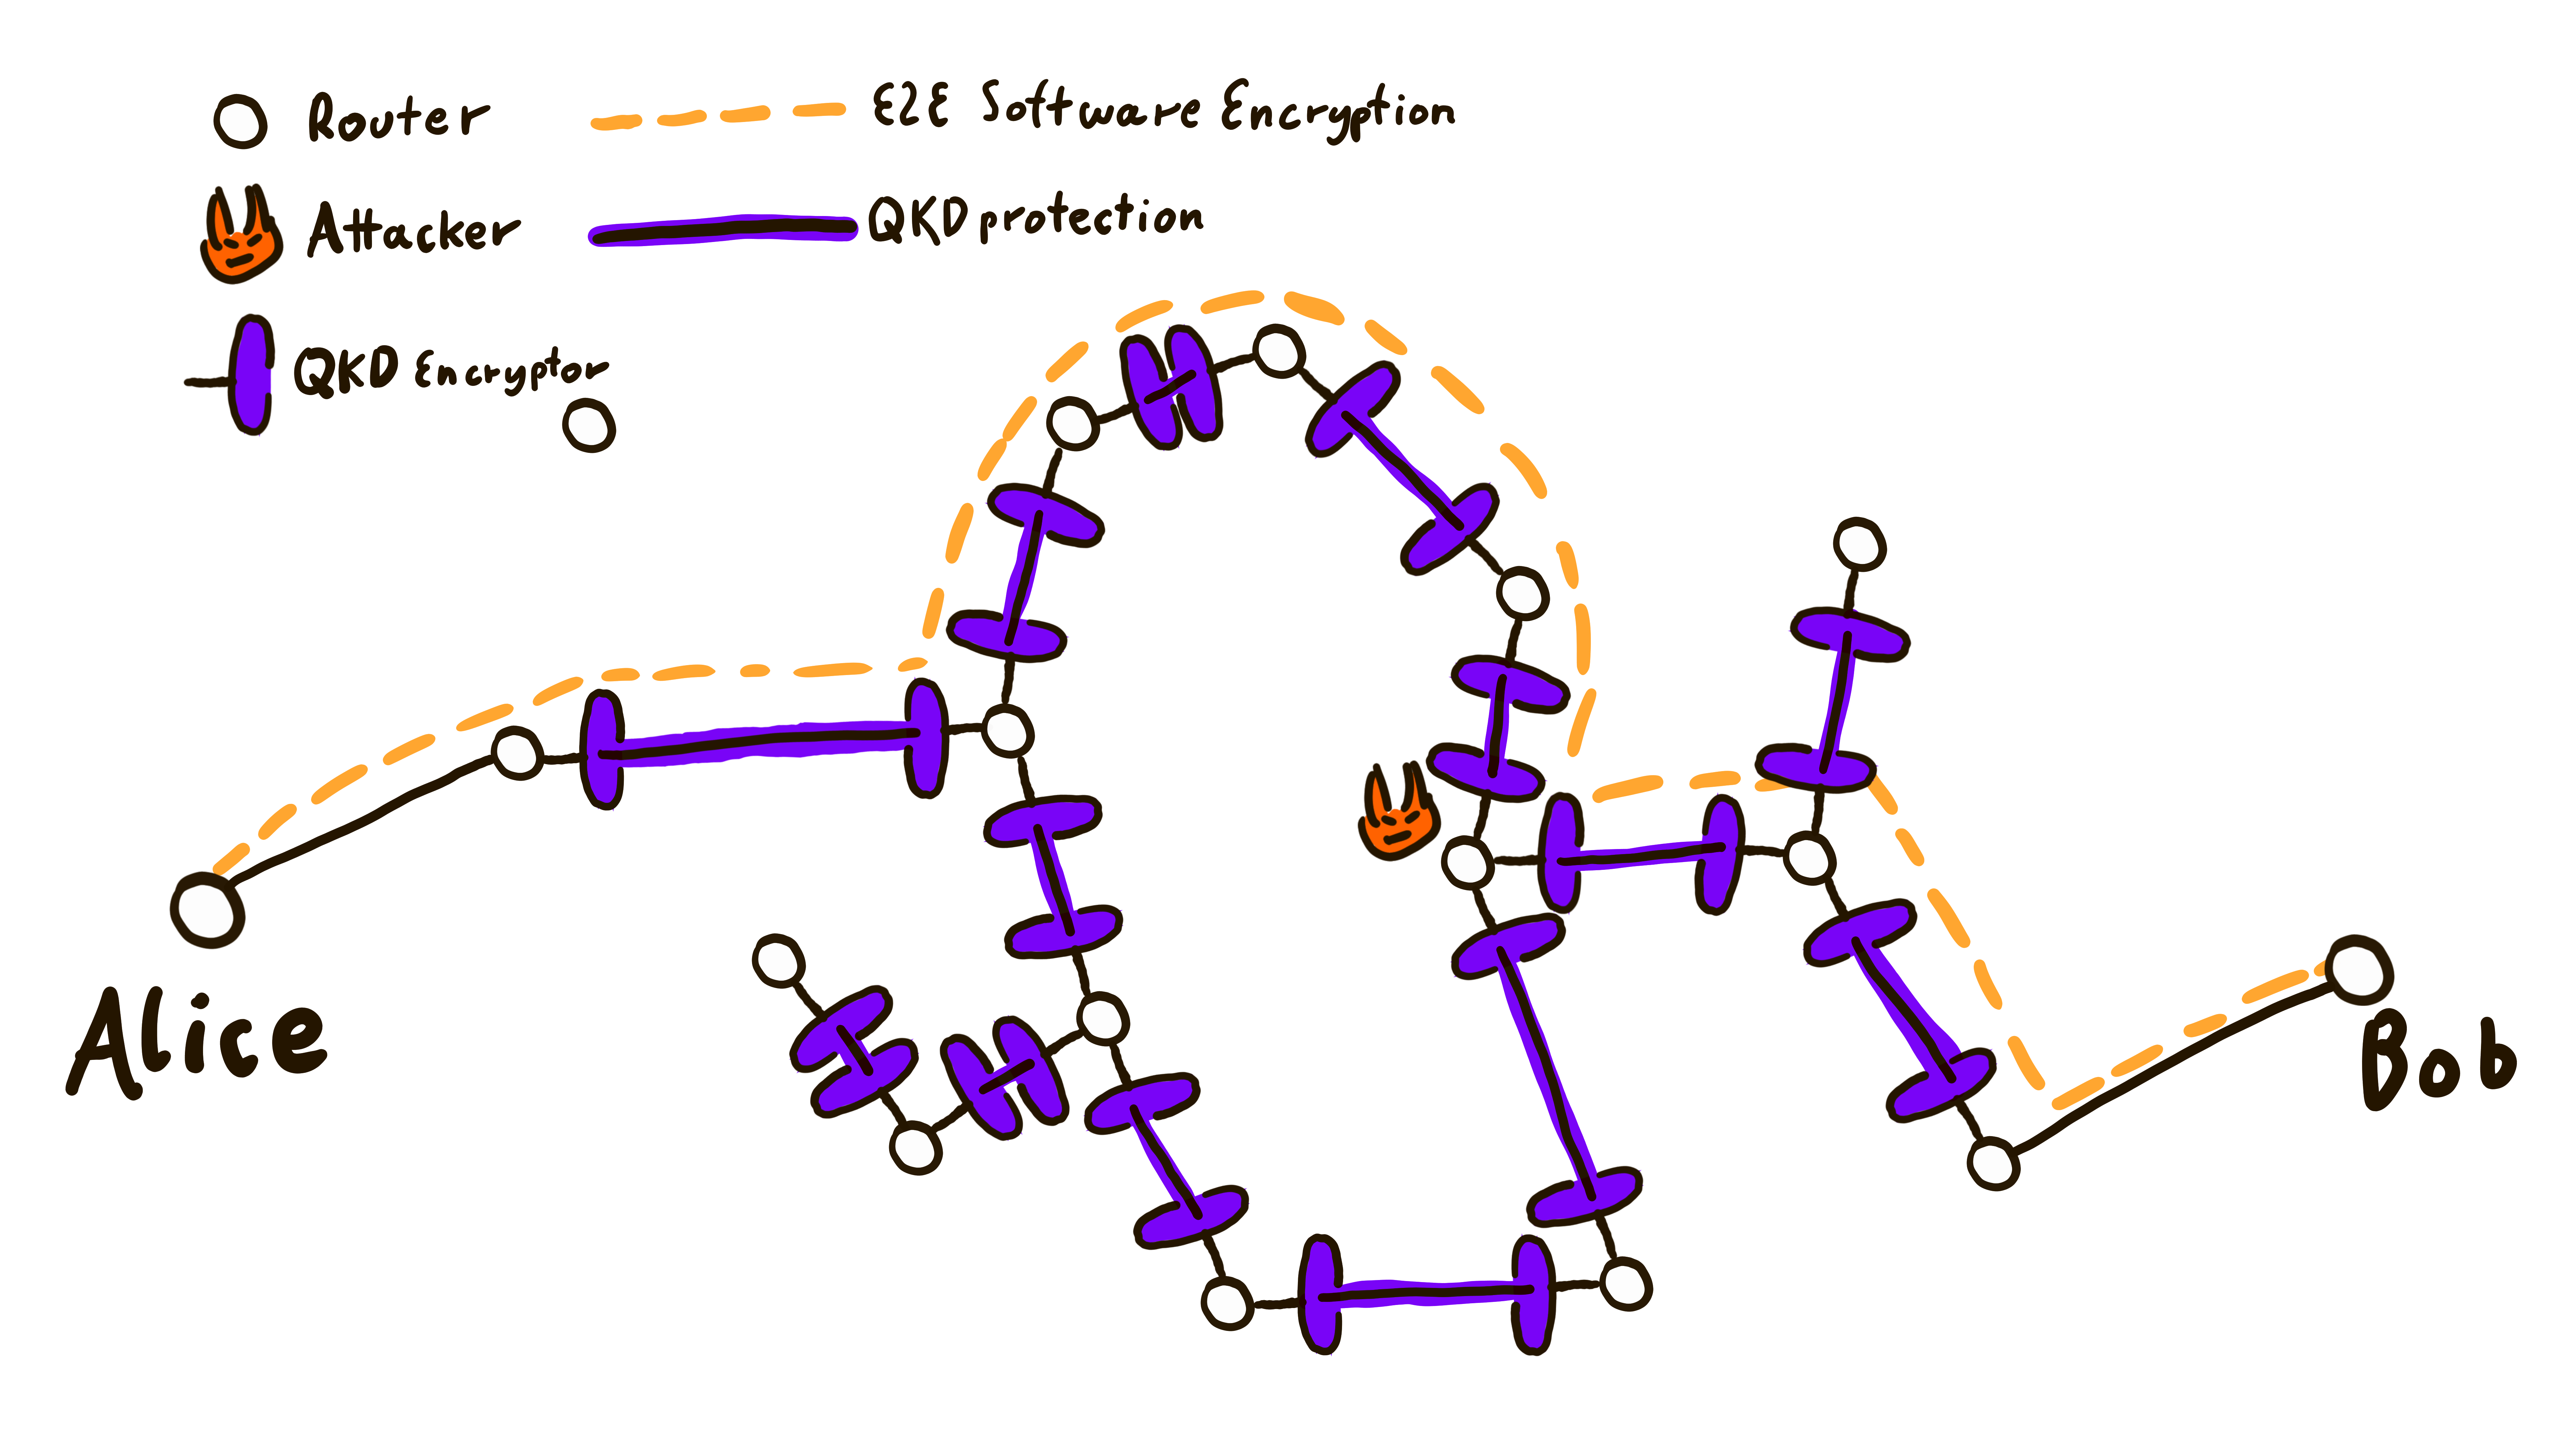
\includegraphics[height=\defaultframetextheight]{graphics/qkd-pqc-network.png}
\end{frame}

\threePillarsSlide
